
%\renewcommand{\theequation}{\theenumi}
%\begin{enumerate}[label=\arabic*.,ref=\thesubsection.\theenumi]
%\numberwithin{equation}{enumi}

\item A=$[a_{ij}]_{mxn}$ is a square matrix,if\\
(A) m$<$n (B)m$>$n (C) m=n (D) None of these\\
\item Which of the given values of x and y make the following pair of matrices equal \myvec{3x+7 &5\\y+1 &2-3x},\myvec{0 &y-2\\8 &4}\\
(A)x=$\frac{-1}{3}$,y=7 \\
 (B) Not possible to find\\
(C) y=7, x=$\frac{-2}{3}$\\
 (D) x=$\frac{-1}{3}$,y=$\frac{-2}{3}$\\
\item The number of all possible matrices of order 3X3 with each entry 0 or 1 is:\\
(A) 27 (B)18 (C)81 (D)512\\
\item Let A=\myvec{2 &4\\3 &2},B=\myvec{1 &3\\-2 &5},C=\myvec{-2 &5\\3 &4}
Find each of the following:\\
(i) A+B  (ii)A-B  (iii)3A-C  (iv)AB  (v)BA\\
\solution
\begin{enumerate}
  \item 
  \item 
  \item 
\begin{align}
    \myvec{2&3&4\\
           3&4&5\\
           4&5&6}\myvec{1&-3&5\\
                        0&2&4\\
                        3&0&5}
    &=\myvec{2+0+12&-6+6+0&10+12+20\\
           3+0+15&-9+8+0&15+16+25\\
           4+0+18&-12+10+0&20+20+30}\\
    &=\myvec{14&0&42\\
             18&-1&56\\
             22&-2&70}
\end{align}

  \item 
\begin{align}
    \myvec{2&3&4\\
           3&4&5\\
           4&5&6}\myvec{1&-3&5\\
                        0&2&4\\
                        3&0&5}
    &=\myvec{2+0+12&-6+6+0&10+12+20\\
           3+0+15&-9+8+0&15+16+25\\
           4+0+18&-12+10+0&20+20+30}\\
    &=\myvec{14&0&42\\
             18&-1&56\\
             22&-2&70}
\end{align}

\end{enumerate}
\item Compute the following:\\
(i)\myvec{a &b\\-b &a}+\myvec{a &b\\b&a} (ii)\myvec{a^2+b^2 &b^2+c^2\\a^2+c^2 &a^2+b^2}+\myvec{2ab &2bc\\-2ac &-2ab} \\
  (iii) \myvec{-1 &4 &-6\\8 &5 &16\\2 &8 &5}+\myvec{12 &7 &6\\8 &0 &5\\3 &2 &4}\\ 
(iv) \myvec{cos^2x &sin^2x\\sin^2x &cos^2x}+\myvec{sin^2x &cos^2x\\cos^2x &sin^2x}\\
\item Compute the indicated products.
\begin{enumerate}
\item \myvec{2 &3 &4\\3 &4 &5\\4 &5 &6}\myvec{1 &-3 &5\\0 &2 &4\\3 &0 &5} 
\item \myvec{2 &1\\3 &2\\-1 &1}\myvec{1 &0 &1\\-1 &2 &1} \\
\item  \myvec{3 &-1 &3\\-1 &0 &2}\myvec{2 &-3\\1 &0\\3 &1}
\end{enumerate}
\solution
\begin{enumerate}
\item 
\begin{align}
    \myvec{2&3&4\\
           3&4&5\\
           4&5&6}\myvec{1&-3&5\\
                        0&2&4\\
                        3&0&5}
    &=\myvec{2+0+12&-6+6+0&10+12+20\\
           3+0+15&-9+8+0&15+16+25\\
           4+0+18&-12+10+0&20+20+30}\\
    &=\myvec{14&0&42\\
             18&-1&56\\
             22&-2&70}
\end{align}

\end{enumerate}
\item If,A=\myvec{1 &2 &-3\\5 &0 &2\\1 &-1 &1},B=\myvec{3 &-1 &2\\4 &2 &5\\2 &0 &3}and C=\myvec{4 &1 &2\\0 &3 &2\\1 &-2 &3},then compute (A+B) and (B-C).Also ,verify that A+(B-C)=(A+B)-C.\\
\solution
From the given information, 
%
\begin{align}
    \vec{B-A}=\myvec{1\\2\\3}-\myvec{1\\1\\1} = \myvec{0\\1\\2}\\
    \vec{C-A}=\myvec{2\\3\\1}-\myvec{1\\1\\1}=\myvec{1\\2\\0}\\
    \end{align}
The area of a triangle using the vector product is then obtained as
\begin{align}
    \frac{1}{2}\norm{\myvec{\vec{B-A}}\times\myvec{\vec{C-A}}}\\ \frac{1}{2}\norm{\myvec{0\\1\\2}\times \myvec{1\\2\\0}}\\=1
    \end{align}
\item If A=$\myvec{\frac{2}{3} & 1 & \frac{5}{3}\\ \frac{1}{3} & \frac{2}{3} & \frac{4}{3} \\ \frac{7}{3} &2  & \frac{2}{3}}$ and B=$\myvec{\frac{2}{5} & \frac{3}{5} &1 \\ \frac{1}{5} & \frac{2}{5} & \frac{4}{5}\\ \frac{7}{5} & \frac{6}{5} & \frac{2}{5}}$,then compute 3A-5B.\\
\solution
From the given information, 
%
\begin{align}
\vec{B-A}&=\myvec{2\\3\\5}-\myvec{1\\1\\2} = \myvec{1\\2\\3}\\
\vec{C-A}&=\myvec{1\\5\\5}-\myvec{1\\1\\2}=\myvec{0\\4\\3}
\end{align}
The area of a triangle using the vector product is then obtained as
\begin{align}
        \frac{1}{2}\norm{\myvec{\vec{B-A}}\times\myvec{\vec{C-A}}} \\=\frac{1}{2}\norm{\myvec{1\\2\\3}\times \myvec{0\\4\\3}}\\=\frac{17}{2}
    \end{align}
\item Find x and y,if 2 \myvec{1 &3\\0 &x}+\myvec{y &0\\1 &2}=\myvec{5 &6\\1 &8}\\
\solution
\begin{align}
    2\myvec{1&3\\0&x} + \myvec{y&0\\1&2} &= \myvec{5&6\\1&8}\\
    \implies \myvec{2&6\\0&2x} + \myvec{y&0\\1&2} &= \myvec{5&6\\1&8}\\
    \implies \myvec{2+y&6+0\\0+1&2x+2} &= \myvec{5&6\\1&8}\\
    \implies 2+y=5,\; 2x&+2=8\\
    \implies y=3,\; x&=3
\end{align}
\item Solve the equation for x,y,z and t,if \\
2\myvec{x &z\\y &t}+3\myvec{1 &-1\\0 &2}=3\myvec{3 &5\\4 &6}\\
\item If x=\myvec{2 \\3}+y\myvec{-1 \\1}=\myvec{10 \\5},find the values of x and y.\\
\solution
%
If solution exists for the given
system of equations then they
said to be consistent, otherwise they are
inconsistent.
The above equations can be expressed as the matrix equation
\begin{align}
\myvec{1 & 2\\2 & 3} \vec{x} = \myvec{2\\3}
\end{align}
%
The augmented matrix for the above equation and row reducing as follows
\begin{align}
\myvec{1 & 2 & 2 \\ 2 & 3 & 3}  \xleftrightarrow[]{R_2\rightarrow R_2-2R_1} \myvec{1 & 2 & 2 \\ 0 & -1 & -1}\\
\xleftrightarrow[]{R_1\rightarrow R_1+2R_2}
\myvec{1 & 0 & 0\\0 & -1 & -1}\label{aug/2/70/a}\\
\implies\text{Rank}\myvec{1&2\\2&3}=\text{Rank}\myvec{1&2&2\\2&3&3}=2
\end{align}
Here, $Rank(A)=Rank(A|B)$. Therefore, the system is consistent. Also, there exist a unique solution as $Rank(A)=n$ (number of unknown).\\ 
From equation \eqref{aug/2/70/a}, we get:
\begin{align}
    \vec{x}=\myvec{0\\1}
\end{align}
Plotting the lines and the intersection point in Fig.\ref{aug/2/70/b}
\begin{figure}[htp]
\centering
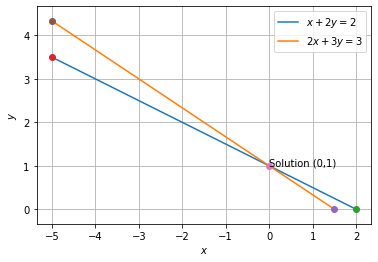
\includegraphics[width=\columnwidth]{solutions/aug/2/70/a_2.png}
\caption{Lines and their intersection denoting the solution}
\label{aug/2/70/b}
\end{figure}
%
$\therefore$ The given system of equation is consistent with unique solution of,
$$\myvec{x\\y}=\myvec{0\\1}$$


\item Given 3\myvec{x &y\\z &w}=\myvec{x &6\\-1 &2w}+\myvec{4 &x+y\\z+w &3},find the values of x,y,z and w.\\


Assume X,Y,Z,W and P are matrices of orders $2\times n$,$3 \times k$,$2\times p$,$n\times 3$ and $p\times k$,respectively.\\
Choose the correct answer in Exercise 31 and 32.\\
\item The restriction on n,k and p so that PY+WY will be defined are:\\
(A)k=3,p=n\\
 (B)k is arbitrary,p=2 \\
 (C)p is arbitrary,k=3 \\
 (D)k=2,p=3\\
\item If n=p,then the order of the matrix 7X-5Z is:\\
(A)$p \times 2$ (B)$2 \times n$ (C)$n \times 3$ (D)$p \times n$\\
\item Find the transpose of each of the following matrices:\\
(i)\myvec{5\\ \frac{1}{2} \\-1}\\ (ii)\myvec{1 &-1\\2 &3}\\ (iii)\myvec{-1 &5 &6\\\sqrt{3} &5 &6\\2 &3 &-1}\\
\item If A=\myvec{-1 &2 &3\\5 &7 &9\\-1 &1 &1} and B=\myvec{-4 &1 &-5\\1 &2 &0\\1 &3 &1},then verify that\\
(i)$(A+B)^{'}=A^{'}+B^{'}$ \\(ii) $(A-B)^{'}=A^{'}-B^{'}$\\
\solution
\begin{enumerate}
  \item 
  \item Given equation of the line, 
\begin{align}
\myvec{k-3 & -(4-k^2)}\vec{x}+k^2-7k+6=0\label{oct/2/106/eq:1}\end{align}
of a general line equation \begin{align}{\vec{nx} = c}\end{align}\newline
here \begin{align}{\vec{n} =\myvec{k-3 & -\{4-k^2\}}}\newline\end{align}
and \begin{align}{c = -k^2+7k-6}\end{align}
\begin{enumerate}[label=\emph{\alph*)}]
\item Parallel to x-axis
\begin{align}
\vec{n}=\myvec{0 & 1}\end{align}if the line is parallel to x-axis
Equation of x-axis is \begin{align}\begin{split}\myvec{1 & 0}\vec{x}& =0\\
 \myvec{1 & 0}\myvec{k-3\\-\{4-k^2\}} & = 0 \label{oct/2/106/eq1}\\
  k-3 & = 0\\
    \implies k & =3
\end{split}\end{align}
Substituting $k=3$ in \eqref{oct/2/106/eq:1}
Equation of line is,
\begin{align}
     \myvec{0 & 5}\vec{x}=6
\end{align}
 
\item Parallel to y-axis
 \begin{align}\vec{n} & =\myvec{1 & 0} \end{align} if the line is parallel to y-axis Equation of y-axis is  \begin{align}\begin{split}\myvec{0 & 1}\vec{x} & =0\\
\myvec{0 & 1}\myvec{k-3\\-(4-k^2)} & = 0\\ \label{oct/2/106/eq1}
 4-k^2 & =0\\
 \implies k & =\pm2
\end{split}
\end{align}
Substituting $k=2$ in \eqref{oct/2/106/eq:1}.
Equation of line is,
\begin{align}
     \myvec{-1 & 0}\vec{x} & = 4
\end{align}
Substituting $k=-2$ in \eqref{oct/2/106/eq:1}.
Equation of line is,
\begin{align}
  \myvec{-5 & 0}\vec{x} & =-24
\end{align}
\item Passing through origin 
${c = 0}$ if the line passes through origin
Equation of line when passing through origin is 
\begin{align}
\vec{n}^\top\vec{x} & =0
\end{align}
Hence
\begin{align} \label{oct/2/106/eq1}
\begin{split}
-k^2+7k-6 & = 0\\
 & = -k^2+k+6k-6\\
 & =(k-1)(k-6)\\
\implies k&=1, k=6
\end{split}
\end{align}
Substituting $k=1$ in \eqref{oct/2/106/eq:1}.
The equation of line is,
\begin{align}
\myvec{-2&-3}\vec{x} = 0
\end{align}
Substituting $k=6$ in \eqref{oct/2/106/eq:1}.
The equation of line is,
\begin{align}
  \myvec{3 & 32}\vec{x} = 0
\end{align}
\end{enumerate}
\begin{figure}[!h]
         \centering
         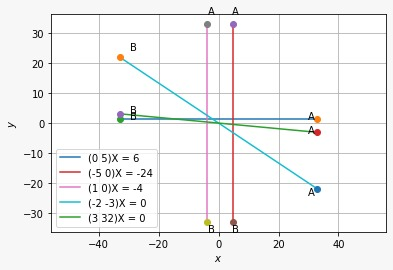
\includegraphics[width=\columnwidth]{solutions/oct/2/106/figure L.jpeg}
         \caption{Plot of line equations}
         \label{oct/2/106/fig:x cubed graph}
\end{figure}

\end{enumerate}
\item If $A^{'}$=\myvec{3 &4\\-1 &2\\0 &1} and B=\myvec{-1 &2 &1\\1 &2 &3},then verify that\\
(i) $(A+B)^{'}=A^{'}+B^{'}$ (ii)$(A-B)^{'}=A^{'}-B^{'}$
\\
\solution
\begin{enumerate}
  \item %
If solution exists for the given
system of equations then they
said to be consistent, otherwise they are
inconsistent.
The above equations can be expressed as the matrix equation
\begin{align}
\myvec{1 & 2\\2 & 3} \vec{x} = \myvec{2\\3}
\end{align}
%
The augmented matrix for the above equation and row reducing as follows
\begin{align}
\myvec{1 & 2 & 2 \\ 2 & 3 & 3}  \xleftrightarrow[]{R_2\rightarrow R_2-2R_1} \myvec{1 & 2 & 2 \\ 0 & -1 & -1}\\
\xleftrightarrow[]{R_1\rightarrow R_1+2R_2}
\myvec{1 & 0 & 0\\0 & -1 & -1}\label{aug/2/70/a}\\
\implies\text{Rank}\myvec{1&2\\2&3}=\text{Rank}\myvec{1&2&2\\2&3&3}=2
\end{align}
Here, $Rank(A)=Rank(A|B)$. Therefore, the system is consistent. Also, there exist a unique solution as $Rank(A)=n$ (number of unknown).\\ 
From equation \eqref{aug/2/70/a}, we get:
\begin{align}
    \vec{x}=\myvec{0\\1}
\end{align}
Plotting the lines and the intersection point in Fig.\ref{aug/2/70/b}
\begin{figure}[htp]
\centering
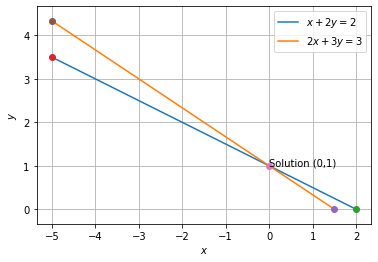
\includegraphics[width=\columnwidth]{solutions/aug/2/70/a_2.png}
\caption{Lines and their intersection denoting the solution}
\label{aug/2/70/b}
\end{figure}
%
$\therefore$ The given system of equation is consistent with unique solution of,
$$\myvec{x\\y}=\myvec{0\\1}$$


  \item 
\end{enumerate}

\item If$ A^{'}$=\myvec{-2 &3\\1 &2} and B=\myvec{-1 &0\\1 &2},then find that $(A+2B)^{'}$\\

  \item (i) Show that the matrix A=\myvec{1 &-1&5\\-1 &2 &1\\5 &1 &3} is a symmetric matrix.\\
  (ii) Show that the matrix A=\myvec{0 & 1 &-1\\-1 &0 &1\\1&-1 &0} is a skew symmetric matrix.\\
  \solution
  \begin{enumerate}
    \item Given,
    \begin{align}
    \label{aug/2/19/eq:1}
        \vec{A}=\myvec{1 & -1 & 5\\ -1 & 2 & 1\\5 & 1 & 3}
    \end{align}
    Transposing the matrix,
    \begin{align}
        \label{aug/2/19/eq:2}
        \vec{A}^\top=\myvec{1 & -1 & 5 \\-1 & 2 & 1\\5 & 1 &3}
    \end{align}
    Using \eqref{aug/2/19/eq:1} and \eqref{aug/2/19/eq:2} we get,
    \begin{align}
        \vec{A}=\vec{A}^\top
    \end{align}
    %\begin{center}
        $\therefore \vec{A}$ is symmetric matrix. 
    %\end{center}
        
    \item Given,
    \begin{align}
    \label{aug/2/19/eq:4}
        \vec{A}=\myvec{0 & 1 & -1\\ -1 & 0 & 1\\1 & -1 & 0}
    \end{align}
    Transposing the matrix,
    \begin{align}
        \label{aug/2/19/eq:5}
        \vec{A}^\top=\myvec{0 & -1 & 1 \\1 & 0 & -1\\-1 & 1 & 0}
    \end{align}
    Using \eqref{aug/2/19/eq:4} and \eqref{aug/2/19/eq:5} we get,
    \begin{align}
        \vec{A}=-\vec{A}^\top
    \end{align}
    %\begin{center}
        $\therefore \vec{A}$ is skew symmetric matrix. 
    %\end{center}
    \end{enumerate}
  \item For the matrix A=\myvec{1 &5\\6 &7},verify that\\
  (i)$(A+A^{'})$ is a symmetric matrix\\
  (ii)$(A-A^{'})$ is a skew symmetric matrix\\
  \solution
  From the given information, 
\begin{align}
\vec{P} &= \myvec{3&-2}\myvec{\vec{a}\\\vec{b}}\\
\vec{Q} &= \myvec{1&1}\myvec{\vec{a}\\\vec{b}}
\\
\implies \myvec{\vec{P}\\\vec{Q}} &= \myvec{3 & -2\\1 & 1}\myvec{\vec{a} \\ \vec{b}}
\end{align}
\begin{enumerate}
\item 
For  internal division, using section formula, 
\begin{align}
\vec{R} &= \myvec{\frac{m}{m+n} & \frac{n}{m+n}}\myvec{\vec{P}\\\vec{Q}}\\
&= \myvec{\frac{m}{m+n} & \frac{n}{m+n}}\myvec{3 & -2\\1 & 1}\myvec{\vec{a} \\ \vec{b}}
\end{align}
For ratio 2 : 1,
\begin{align}
\vec{R} &= \myvec{\frac{2}{2+1} & \frac{1}{2+1}}\myvec{\vec{P}\\\vec{Q}}\\
&= \myvec{\frac{2}{3}&\frac{1}{3}}\myvec{3 & -2\\1 & 1}\myvec{\vec{a} \\ \vec{b}}\\
&= \myvec{\frac{7}{3} & -1}\myvec{\vec{a} \\ \vec{b}}\\
\implies \vec{R} &= \frac{7}{3}\vec{a} - \vec{b}
\end{align}

\item Similarly,  for external division,
\begin{align}
\vec{R} &= \myvec{\frac{m}{m-n} & \frac{n}{m-n}}\myvec{\vec{P}\\\vec{Q}}\\
&= \myvec{\frac{m}{m-n} & \frac{n}{m-n}}\myvec{3 & -2\\1 & 1}\myvec{\vec{a} \\ \vec{b}}
\end{align}
For ratio 2 : 1,
\begin{align}
\vec{R} &= \myvec{\frac{2}{2-1} & -\frac{1}{2-1}}\myvec{\vec{P}\\\vec{Q}}\\
&= \myvec{2 & -1}\myvec{3 & -2\\1 & 1}\myvec{\vec{a} \\ \vec{b}}\\
&= \myvec{5 & -5}\myvec{\vec{a} \\ \vec{b}}\\
\vec{R} &= 5\vec{a} - 5\vec{b}
\end{align}
%
\end{enumerate}
  \item Find $\frac{1}{2}(A+A^{'}) $and $\frac{1}{2}(A-A^{'})$,when A=\myvec{0 &a &b\\-a &0 &c\\-b &-c &0}\\
  \item Express the following matrices as the sum of a symmetric and a skew symmetric matrix:\\
  (i) \myvec{3 &5\\1 &1} \\(ii) \myvec{6 &-2 &2\\-2 &3 &-1\\2 &-1 &3} \\
  (iii) \myvec{3 &3 &-1\\-2 &-2 &1\\-4 &-5 &2}\\ (iv) \myvec{1 &5\\-1 &2}\\
  \begin{enumerate}
    \item 
\begin{table}[!ht]
\centering
\resizebox{\columnwidth}{!}{\begin{tabular}{|c|c|c|c|} 
\hline
kind of  cake & No.of cakes & Flour& Fat\\
\hline
1st & x & 200g  &  25g \\ 
\hline
2nd& y& 100g&  50g  \\ 
\hline
Total& x+y& 5 kg=5000g&1kg=1000g \\ 
\hline
\end{tabular}}
\caption{Ingredients used in making the cake is flour and fat }
\label{opt/13/tab:table1}
\end{table}
Let the  1st kind  be $x$ and the 2nd kind be $y$  such that 
\begin{align}
x \geq 0 \\
y \geq 0 
\end{align}
According to the question,
\begin{align}
2{x} + {y} \leq 50
\\
{x} + 2{y} \leq 40
\end{align}
$\therefore$ Our problem is
\begin{align}
\max_{\vec{x}} Z &= \myvec{1& 1}\vec{x}\\
s.t. \quad \myvec{2 & 1 \\ 1& 2}\vec{x} &\preceq \myvec{50\\40} 
\end{align}
Lagrangian function is given by
\begin{equation}
\begin{aligned}
&L(\vec{x},\boldsymbol{\lambda}) \\ &= \myvec{1 & 1}\vec{x}+\lcbrak{\sbrak{\myvec{2 & 1}\vec{x}-50}} \\ &+ \sbrak{\myvec{1 & 2}\vec{x}-40}\\ &+ \sbrak{\myvec{-1 & 0}\vec{x}} +\rcbrak{\sbrak{\myvec{0 & -1}\vec{x}}}\boldsymbol{\lambda}
\end{aligned}
\end{equation}
where,
\begin{align}
\boldsymbol{\lambda} &= \myvec{\lambda_1 \\ \lambda_2 \\ \lambda_3 \\ \lambda_4 \\ \lambda_5 \\ \lambda_6}
\end{align}
Now,
\begin{align}
\nabla L(\vec{x},\boldsymbol{\lambda}) &= \myvec{1+ \myvec{2 & 1 & -1 & 0 }\boldsymbol{\lambda}\\ 1+\myvec{1 & 2 & 0 & -1}\boldsymbol{\lambda} \\ \myvec{2 & 1}\vec{x}-50\\ \myvec{1& 2}\vec{x}-40 \\  \myvec{-1 & 0}\vec{x} \\ \myvec{0 & -1}\vec{x}}
\end{align}
$\therefore$ Lagrangian matrix is given by
\begin{align}
\myvec{0 & 0 & 2 & 1& -1 & 0 \\ 0 & 0 & 1 & 2  & 0 & -1 \\ 2 & 1 & 0 & 0 & 0 & 0 \\ 1 & 2 & 0 & 0 & 0 & 0  \\ -1 & 0 & 0 & 0 & 0 & 0  \\ 0 & -1 & 0 & 0 & 0 & 0 }\myvec{\vec{x} \\ \boldsymbol{\lambda} } &= \myvec{-1 \\ -1 \\ 50\\ 4 0\\ 0 \\0 }
\end{align}
Considering $\lambda_1,\lambda_2$ as only active multiplier,
\begin{align}
\myvec{0 & 0 & 2 & 1 \\ 0 & 0 & 1 & 2 \\ 2 & 1 & 0 & 0 \\ 1 & 2 & 0 & 0}\myvec{\vec{x}\\ \boldsymbol{\lambda}} &= \myvec{-1 \\ -1 \\ 5 0\\ 40}
\end{align}
resulting in,
\begin{align}
\myvec{\vec{x} \\ \boldsymbol{\lambda}} &= \myvec{0 & 0 & 2 & 1 \\ 0 & 0 & 1 & 2 \\ 2 & 1 & 0 & 0 \\ 1& 2 & 0 & 0}^{-1}\myvec{-1 \\ -1 \\ 50 \\ 40}
\\
\implies   \myvec{\vec{x} \\ \boldsymbol{\lambda}} &= \myvec{0 & 0 & \frac{2}{3} & \frac{-1}{3} \\ 0 & 0 & \frac{-1}{3} & \frac{2}{3} \\ \frac{2}{3} & \frac{-1}{3} & 0 & 0 \\ \frac{-1}{3} & \frac{2}{3} & 0 & 0}\myvec{-1 \\ -1 \\ 50 \\ 40}
\\
\implies \myvec{\vec{x} \\ \boldsymbol{\lambda}} &= \myvec{20 \\ 10 \\ -0.3 \\ -0.3 }
\end{align}
$\because \boldsymbol{\lambda}=\myvec{-0.3 \\ -0.3} \succ \vec{0} $
\\
$\therefore$ Optimal solution is given by
\begin{align}
    \vec{x} &= \myvec{20\\10} \\
    Z &= \myvec{1& 1}\vec{x} \\
    &= \myvec{1 & 1}\myvec{20 \\ 10} \\
    &= 60
\end{align}
By using cvxpy in python ,
\begin{align}
    \vec{x}=\myvec{20\\10}\\
    Z = 60
\end{align}
Hence No.of cakes \boxed{x=20} 1st kind and  .of cakes \boxed{y=10} 2nd kind should be used to maximum No. of cakes \boxed{Z=60}.  This is
verified in Fig. \ref{opt/13/fig: Graphical Solution}.	
%
\begin{figure}[!ht]
\centering
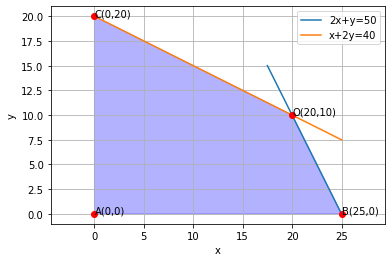
\includegraphics[width=\columnwidth]{solutions/su2021/2/13/Figure9.png}
\caption{Graphical Solution}
\label{opt/13/fig: Graphical Solution}	
\end{figure}

    \item Let A be the given matrix\\
\begin{align}
    \vec{A}&=\myvec{6&-2&2\\-2&3&-1\\2&-1&3}\\
    \vec{A}^T&=\myvec{6&-2&2\\-2&3&-1\\2&-1&3}\\
    \implies \vec{A}&=\vec{A}^T\label{aug/2/22/2eq1}
\end{align}
Since, $\vec{A}$ is a symmetric matrix the skew symmetric matrix would be 0

  \end{enumerate}
  Choose the correct answer in question number 43 and 44\\
  \item If A,B are symmetric matrices of same order,then AB-BA is a\\
  (A)Skew symmetric matrix \\(B)Symmetric matrix\\
  (C)Zero matrix \\ (D)Identity matrix\\
  
  
  \item\myvec{1 &3\\2 &7}\\
  \item\myvec{2 &3\\5 &7}\\
  \item\myvec{2 &1\\7 &4}\\
  \item \myvec{2 &5\\1 &3}\\
  \item \myvec{3 &1\\5 &2}\\
  \item \myvec{4 &5\\3 &4}\\
  \item \myvec{3 &10\\2 &7}\\
  \item \myvec{3 &-1\\-4 &2}\\
  \item \myvec{2 &-6\\1 &-2}\\
  \item \myvec{6 &-3\\-2 &1}\\
  \item \myvec{2 &-3\\-1 &2}\\
  \item \myvec{2 &1\\4 &2}\\
  
  \item Matrices Aand B will be inverse of each other only if\\
  (A)AB=BA (B)AB=BA=0\\
  (C)AB=0,BA=I (D)AB=BA=I\\
  
  \item Let A=\myvec{0 &1\\0 &0},show that \\$(aI+bA)^{n}=a^{n}I+na^{n-1}bA$,where I is the identity matrix of order 2 and $n \epsilon N$\\

  \item If A and B are symmetric matrices,prove that AB-BA is a skew symmetric matrix.\\
  
  \item If A and B are square matrices of the same order such that AB=BA,then prove by indication that $AB^{n}=B^{n}A$.Further prove that $(AB)^{n}=A^{n}B^{n}$ for all $n \epsilon N$.\\
  Choose the correct answer in the following questions:\\

\item Balance the following chemical equation
\begin{align}\label{1}
    BaCl_2 + H_2SO_4 \xrightarrow{} BaSO_4 + HCl
\end{align}
    \item If A=\myvec{1 &2 &3\\2 &3 &1} and B=\myvec{3 &-1 &3\\-1 &0 &2}, then find 2A-B.\\
    \item If A=\myvec{8 &0\\4 &-2\\3 &6} and B=\myvec{2 &-2\\4 &2\\-5 &1}, then find the matrix X, such that 2A+3X=5B.\\
    \solution
    From the given info, 
 \begin{align}
 \implies \vec{X}=\frac{\vec{5B}-\vec{2A}}{3}\\
 \vec{X}&=\myvec{-2 & -10/3 \\ 4 & 14/3 \\ -31/3 & -7/3}
\end{align}

    \item Find X and Y, if X+Y=\myvec{5 &2\\0 &9} and \\X-Y=\myvec{3 &6\\0 &-1}.\\
    \item Find the values of x and y from the following equation:\\
    2\myvec{x &5\\7 &y-3} + \myvec{3 &-4\\1 &2} = \myvec{7 &6\\15 &14}\\
     
    

   
    \item  Find AB, if A=\myvec{6 &9\\2 &3} and B=\myvec{2 &6 &0\\7 &9 &8}.\\
    \item  If A=\myvec{1 &-2 &3\\-4 &2 &5\\} and B=\myvec{2 &3\\4 &5\\2 &1}, then find AB,BA.Show that AB$\neq$BA.
    \\
    \solution
    \input{}

   
     \item If A=\myvec{1 &0 \\0 &-1} and  B=\myvec{0 &1\\1 &0}, then find AB,BA. Show that AB$\neq$BA\\
     \solution
     Performing respective matrix multiplications,
\begin{align}
    \vec{AB} &= \myvec{1 & 0\\ 0 & -1}\times\myvec{0 & 1\\1 & 0}\\
    \vec{AB} &= \myvec{0 & 1\\-1 & 0}\\
    \text{Similarly,}\notag \\
    \vec{BA} &= \myvec{0 & 1\\1 & 0}\times\myvec{1 & 0\\ 0 & -1}\\
    \vec{BA} &= \myvec{0 & -1\\1 & 0}\\
    \\\therefore \vec{AB} &\neq \vec{BA}
\end{align}
     
   
    \item Find AB, if A=\myvec{0 &-1\\0 &2} and B=\myvec{3 &5\\0 &0}\\
    \solution $AB = 0$.

     
   
    \item If A=\myvec{1 &1 &-1\\2 &0 &3\\3 &-1 &2}, B=\myvec{1 &3\\0 &2\\-1 &4} and C=\myvec{1 &2 &3 &-4\\2 &0 &-2 &1}, find\\A(BC),(AB)C and show that (AB)C=A(BC) \\   
    
     \item If A=\myvec{0 &6 &7\\-6 &0 &8\\7 &-8 &0}, B=\myvec{0 &1 &1\\1 &0 &2\\1 &2 &0},C=\myvec{2\\-2\\3}\\Calculate AC,BC and (A+B)C=AC+BC\\
     \solution
     Let the balanced version of \eqref{matrix/50/eq1} be
\begin{align}
   x_{1}NaOH + x_{2}H_2SO_4 \xrightarrow{} 
   x_{3}Na_2SO_4 + x_{4}H_2O \label{matrix/50/eq2}
\end{align}
which results in the following equations:
\begin{align}
    (x_{1}-2x_{3}) Na= 0\\
    (x_{1}+4x_{2}-4x_{3}-x_{4}) O= 0\\
    (x_{1}+2x_{2}-2x_{4}) H=0\\
    (x_{2}-x_{3}) S= 0
\end{align}
which can be expressed as
\begin{align}
    x_{1}+ 0.x_{2}- 2x_{3}+ 0.x_{4} = 0\\
    x_{1}+ 4x_{2}- 4x_{3}- x_{4} = 0\\
    x_{1}+ 2x_{2}+ 0.x_{3}- 2x_{4} = 0\\
    0.x_{1}+ x_{2}- x_{3}+ 0.x_{4} = 0
\end{align}
resulting in the matrix equation
\begin{align}
    \myvec{1 & 0 & -2 & 0\\
           1 & 4 & -4 & -1\\
           1 & 2 & 0 & -2\\
           0 & 1 & -1 & 0}\vec{x}
           =\vec{0}    \label{matrix/50/eq3}
\end{align}
where,
\begin{align}
   \vec{x}= \myvec{x_{1}\\x_{2}\\x_{3}\\x_{4}}
\end{align}
\eqref{matrix/50/eq3} can be reduced as follows:
\begin{align}
    \myvec{1 & 0 & -2 & 0\\
           1 & 4 & -4 & -1\\
           1 & 2 & 0 & -2\\
           0 & 1 & -1 & 0}
    \xleftrightarrow[R_{3}\leftarrow R_3-R_{1}]{R_{2}\leftarrow R_2- R_1}
    \myvec{1 & 0 & -2 & 0\\
           0 & 4 & -2 & -1\\
           0 & 2 & 2 & -2\\
           0 & 1 & -1 & 0}\\
    \xleftrightarrow{R_2 \leftarrow \frac{R_2}{4}}
    \myvec{1 & 0 & -2 & 0\\
          0 & 1 & -\frac{1}{2} & -\frac{1}{4}\\
          0 & 2 & 2 & -2\\
          0 & 1 & -1 & 0}\\
    \xleftrightarrow[R_4 \leftarrow R_4 - R_2]{R_3 \leftarrow R_3 - 2R_2}
    \myvec{1 & 0 & -2 & 0\\
           0 & 1 & -\frac{1}{2} & -\frac{1}{4}\\
           0 & 0 & 3 & -\frac{3}{2}\\
           0 & 0 & -\frac{1}{2} & \frac{1}{4}}\\
    \xleftrightarrow{R_3 \leftarrow \frac{R_3}{3}}
    \myvec{1 & 0 & -2 & 0\\
           0 & 1 & -\frac{1}{2} & -\frac{1}{4}\\
           0 & 0 & 1 & -\frac{1}{2}\\
           0 & 0 & -\frac{1}{2} & \frac{1}{4}}\\
    \xleftrightarrow[R_{4}\leftarrow R_4+\frac{R_3}{2}]{R_{2}\leftarrow R_2+ \frac{R_3}{2}}
    \myvec{1 & 0 & -2 & 0\\
           0 & 1 & 0 & -\frac{1}{2}\\
           0 & 0 & 1 & -\frac{1}{2}\\
           0 & 0 & 0 & 0}\\
    \xleftrightarrow{R_1 \leftarrow R_1+2R_3}
    \myvec{1 & 0 & 0 & -1\\
           0 & 1 & 0 & -\frac{1}{2}\\
           0 & 0 & 1 & -\frac{1}{2}\\
           0 & 0 & 0 & 0}
\end{align}
Thus,
\begin{align}
    x_1=x_4, x_2= \frac{1}{2}x_4, x_3=\frac{1}{2}x_4\\
    \implies \quad\vec{x}= x_4\myvec{1\\ \frac{1}{2}\\ \frac{1}{2}\\1} 
\end{align} 
by substituting $x_4= 2$
\begin{align}
    \vec{x}=\myvec{2\\1\\1\\2}
\end{align}
Hence, \eqref{matrix/50/eq2} finally becomes
\hfill\break
%\vspace{5mm}  finally becomes
\begin{align}
    2 NaOH + H_2SO_4 \xrightarrow{} 
    Na_2SO_4 + 2 H_2O
\end{align}

    
    

\item If A=$\myvec{3 &\sqrt{3} &2\\4 &2 &0}$ and B=$\myvec{2 &-1 &2\\1 &2 &4}$, verify that\\
(i) $(A^{'})^{'}=A$\\ (ii)$(A+B)^{'}=A^{'}+B^{'}$,\\ (iii) $(kB)^{'}=kB^{'}$,where k is any constant.\\
\item If A=$\myvec{-2\\4 \\5}$,B=$\myvec{1 &3 &-6}$, verify that $(AB)^{'}=B^{'}A^{'}$\\
 \solution 
 From the given information,     
\begin{align}    
    \vec{AB} &= \myvec{-2\\4\\5}\myvec{1&3&-6}\\
 &= \myvec{-2&-6&12\\4&12&-24\\5&15&-30}
\end{align}
Hence, 
\begin{align}
\brak{\vec{AB}}^{\top} &=  \myvec{-2&4&5\\-6&12&15\\12&-24&-30}
\end{align}
Also,
\begin{align}
\vec{A}^{\top} &= \myvec{-2&4&5} \\
\vec{B}^{\top} &= \myvec{1\\3\\-6}
\end{align}
Now
\begin{align}
\vec{B}^{\top}\vec{A}^{\top} &= \myvec{1\\3\\-6}\myvec{-2&4&5}\\
&= \myvec{-2&4&5\\-6&12&15\\12&-24&-30}\\
 &= \brak{\vec{AB}}^{\top} 
\end{align}

\item By using elementary operations,find the inverse of the matrix\\
A=$\myvec{1 &2\\2 &-1}$.\\

\item If A=$\myvec{\cos\theta &\sin\theta\\ \-sin\theta &\cos\theta}$,\\then prove that $A^{n}=\myvec{\cos\theta &\sin n\theta\\\-sin n\theta &\cos n\theta}$, n $\in$ N.\\
\item If A and B are symmetric matrices of the same order, then show that AB is symmetric if and only if A and B commute,that AB = BA.\\
\item Let A=$\myvec{2 &-1\\3 &4}$, B=$\myvec{5 &2\\7 &4}$, C=$\myvec{2 &5\\3 &8}$. Find a matrix D such that CD-AB=0. 
\item Find the values of a,b,c and d from the equations: \myvec{a-b &2a+c\\2a-b &3c+d} = \myvec{-1 &5\\0 &13}
\item Show that\\
(i)$\myvec{5 &-1\\6 &7}\myvec{2 &1\\3 &4}\neq\myvec{2 &1\\3 &4}\myvec{5 &-1\\6 &7}$
\\
(ii)$\myvec{1 &2 &3\\0 &1 &0\\1 &1 &0}\myvec{-1 &1 &0\\0 &-1 &1\\2 &3 &4}\neq \myvec{-1 &1 &0\\0 &-1 &1\\2 &3 &4}\myvec{1 &2 &3\\0 &1 &0\\1 &1 &0}$\\
\item If A=\myvec{3 &-2\\4 &-2} and I=\myvec{1 &0\\0 &1},find k\\
 so that $A^2=kA-2I$\\
  \item Find the matrix X so that\\ X\myvec{1 &2 &3\\4 &5 &6}=\myvec{-7 &-8 &-9\\2 &4 &6}\\
  \solution
  Let,
\begin{align}
    \vec{A} &= \myvec{1 & 2 & 3\\ 4 & 5 & 6}\\
    \vec{B} &= \myvec{-7 & -8 & -9\\ 2 & 4 & 6}
\end{align}
Now, multiplying $\vec{A}^\top$ on both sides,
\begin{align}
    \vec{X}\vec{A}\vec{A}^\top &= \vec{B}\vec{A}^\top\\
   \implies \vec{X} &= \vec{B}\vec{A}^\top(\vec{A}\vec{A}^\top)^{-1}
\end{align}
Therefore,
\begin{align}
    \vec{X} &= \myvec{-7 & -8 & -9\\ 2 & 4 & 6} \myvec{1 & 4\\2 & 5\\3 & 6}(\vec{A}\vec{A}^\top)^{-1}\\
            &= \myvec{-50 & -122\\ 28 & 64} \left[\myvec{1 & 2 & 3\\ 4 & 5 & 6} \myvec{1 & 4\\2 & 5\\3 & 6}\right]^{-1}\\
            &= \myvec{-50 & -122\\ 28 & 64}\left[\myvec{14 & 32\\32 & 77}\right]^{-1}\\
            &= \myvec{-50 & -122\\ 28 & 64}\myvec{\cfrac{77}{54}&\cfrac{-16}{27}\\ \cfrac{-16}{27}& \cfrac{7}{27}}\\
            &= \myvec{1 & -2\\2 & 0}
\end{align}
Now, verifying the solution
\begin{align}
    \textit{L.H.S} &= \vec{X}\myvec{1 & 2 & 3\\ 4 & 5 & 6}\\
                 &= \myvec{1 & -2\\2 & 0}\myvec{1 & 2 & 3\\ 4 & 5 & 6}\\
                 &= \myvec{1-8 & 2-10 & 3-12\\4+0 & 4+0 & 6+0}\\
                 &= \myvec{-7 & -8 & -9\\2 & 4 & 6}\\
                 &= \textit{R.H.S}
\end{align}
Hence the matrix $\vec{X}$ is \myvec{1 & -2\\2 & 0}
\item (i) $\begin{vmatrix}a-b-c& 2a& 2a \\ 2b& b-c-a& 2b \\ 2c& 2c& c-a-b\end{vmatrix}$= $(a+b+c)^3$\\
(ii) $\begin{vmatrix}x+y+2z&x&y \\ z&y+z+2x&y \\ z&x&z+x+2y\end{vmatrix}$=$2(x+y+z)^3$
\item $\begin{vmatrix}1&x&x^2 \\ x^2&1&x \\ x&x^2&1\end{vmatrix}$=$(1-x^3)^2$ 
\item $\begin{vmatrix}1+a^2-b^2&2ab&-2b \\ 2ab&1-a^2+b^2&2a \\ 2b&-2a&1-a^2-b^2\end{vmatrix}$=$(1+a^2+b^2)^3$
\item Let 
A=$\begin{bmatrix}
1&\sin\theta&1 \\ -\sin\theta&1&\sin\theta \\ -1&-\sin\theta&1
\end{bmatrix},$ 
where $0\leq \theta \leq 2\Pi.$ Then
\begin{enumerate}
\item Det(A)=0
\item Det(A)$\in(2,\infty)$
\item Det(A)$\in (2,4)$
\item Det(A)$\in [2,4]$
\end{enumerate}
\item $\begin{vmatrix}
1&1+p&1+p+q \\ 2&3+2p&4+3p+2q \\ 3&6+3p&10+6p+3q
\end{vmatrix}$=1\\
\item $\begin{vmatrix}\sin\alpha&\cos\alpha&\cos(\alpha+\delta) \\ \sin\beta&\cos\beta&\cos(\beta+\delta) \\ \sin\gamma&\cos\gamma&\cos(\gamma+\delta)\end{vmatrix}$=0\\
\item Solve the system of equations \\$\frac{2}{x}+\frac{3}{y}+\frac{10}{z}=4$\\$\frac{4}{x}-\frac{6}{y}+\frac{5}{z}=1$\\$\frac{6}{x}+\frac{9}{y}-\frac{20}{z}=2$\\
\item If a,b,c are in A.P, then the determinant\\
 $\begin{vmatrix}
x+2&x+3&x+2a \\ x+3&x+4&x+2b \\x+4&x+5&x+2c
\end{vmatrix}$ is 
\begin{enumerate}
\item 0
\item 1
\item x
\item 2x
\end{enumerate}
\item If x,y,z are nonzero real numbers, then the inverse of matrix 
A=$\begin{bmatrix}
x&0&0 \\ 0&y&0 \\ 0&0&z
\end{bmatrix}$ is 
\begin{enumerate}
\item $\begin{bmatrix} x^{-1}&0&0 \\ 0&y^{-1}&0 \\ 0&0&z^{-1} \end{bmatrix}$ 
\item $xyz\begin{bmatrix} x^{-1}&0&0 \\ 0&y^{-1}&0 \\ 0&0&z^{-1} \end{bmatrix}$ 
\item $\frac{1}{xyz}\begin{bmatrix} x&0&0 \\ 0&y&0 \\ 0&0&z \end{bmatrix}$ 
\item $\frac{1}{xyz}\begin{bmatrix} 1&0&0 \\ 0&1&0 \\ 0&0&1 \end{bmatrix}$ 
\end{enumerate}
\textbf{Examine the consistency of the system of given Equations.}
\item 
$\begin{alignedat}[t]{2}
x+2y&=2 
\\
2x+3y&=3 
\end{alignedat}$
\\
\solution
%
If solution exists for the given
system of equations then they
said to be consistent, otherwise they are
inconsistent.
The above equations can be expressed as the matrix equation
\begin{align}
\myvec{1 & 2\\2 & 3} \vec{x} = \myvec{2\\3}
\end{align}
%
The augmented matrix for the above equation and row reducing as follows
\begin{align}
\myvec{1 & 2 & 2 \\ 2 & 3 & 3}  \xleftrightarrow[]{R_2\rightarrow R_2-2R_1} \myvec{1 & 2 & 2 \\ 0 & -1 & -1}\\
\xleftrightarrow[]{R_1\rightarrow R_1+2R_2}
\myvec{1 & 0 & 0\\0 & -1 & -1}\label{aug/2/70/a}\\
\implies\text{Rank}\myvec{1&2\\2&3}=\text{Rank}\myvec{1&2&2\\2&3&3}=2
\end{align}
Here, $Rank(A)=Rank(A|B)$. Therefore, the system is consistent. Also, there exist a unique solution as $Rank(A)=n$ (number of unknown).\\ 
From equation \eqref{aug/2/70/a}, we get:
\begin{align}
    \vec{x}=\myvec{0\\1}
\end{align}
Plotting the lines and the intersection point in Fig.\ref{aug/2/70/b}
\begin{figure}[htp]
\centering
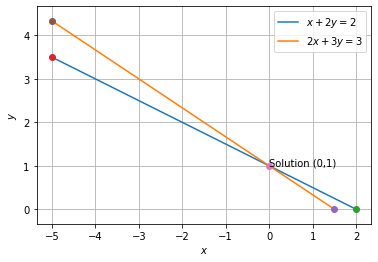
\includegraphics[width=\columnwidth]{solutions/aug/2/70/a_2.png}
\caption{Lines and their intersection denoting the solution}
\label{aug/2/70/b}
\end{figure}
%
$\therefore$ The given system of equation is consistent with unique solution of,
$$\myvec{x\\y}=\myvec{0\\1}$$


\item $\begin{alignedat}[t]{2}
2x-y&=5 
\\
x+y&=4 
\end{alignedat}$
\item Evaluate the determinant
$\begin{vmatrix}0&a&-b\\-a&0&-c\\b&c&0\end{vmatrix}=0$
\\
Find the inverse and QR decomposition of the following.
  \item \myvec{2 &1\\1 &1}\\
  \item\myvec{1 &3\\2 &7}\\
  \item\myvec{2 &3\\5 &7}\\
  \item\myvec{2 &1\\7 &4}\\
  \item \myvec{2 &5\\1 &3}\\
  \item \myvec{3 &1\\5 &2}\\
  \item \myvec{4 &5\\3 &4}\\
  \item \myvec{3 &10\\2 &7}\\
  \item \myvec{3 &-1\\-4 &2}\\
  \item \myvec{2 &-6\\1 &-2}\\
  \item \myvec{6 &-3\\-2 &1}\\
  \item \myvec{2 &-3\\-1 &2}\\
  \item \myvec{2 &1\\4 &2}\\
\item Find the QR decomposition of 
\begin{align}
\vec{A}=\myvec{8&5\\3&2} \label{eq:solutions/decomp/2/29/eq:1}
\end{align}
%%
%
\item Find the QR decomposition of 
\begin{align}
\vec{A}=\myvec{2&5\\1&4} \label{eq:solutions/decomp/2/30/1}
\end{align}

%    \end{document}    

